\chapter{Hydrogen and the s-Block}\label{ch:b1:s-block}

Every phone, laptop and electric car carries a battery whose positive
charges are carried by lithium ions. That lithium comes mostly from two
places: hard-rock mines in Australia and the salt flats of the Andes, where
brine pumped from under the crust is left to evaporate in the sun for
months until lithium salts can be precipitated from it. Lithium is the
first of the \omterm{def:b1:s-block:families}{alkali metals}, the most reactive metals there are, and its
neighbours sodium, potassium, magnesium and calcium supply the bulk
chemicals of industry: caustic soda, soda ash, lime. This chapter opens
the descriptive chemistry of the elements with hydrogen and the \omterm{def:b1:periodicity:table}{s-block},
using the tools of the earlier chapters --- ionisation energies,
\omterm{def:b1:nernst:electrode-potential}{standard potentials}, \omterm{def:b1:precipitation:solubility-product}{solubility products} --- to explain what these
elements do.

\begin{recall}
Ionisation energies and \omterm{def:b1:periodicity:electronegativity}{electronegativity} (\cref{ch:b1:periodicity});
\omterm{def:b1:nernst:electrode-potential}{standard potentials} (\cref{ch:b1:nernst}); \omterm{def:b1:precipitation:solubility-product}{solubility products} and the
precipitation of hydroxides (\cref{ch:b1:precipitation}). The school
volume (grade 10) grouped the elements into families: \omterm{def:b1:s-block:families}{alkali metals},
\omterm{def:b1:s-block:families}{alkaline-earth metals}, halogens, noble gases.
\end{recall}

\begin{omfigure}
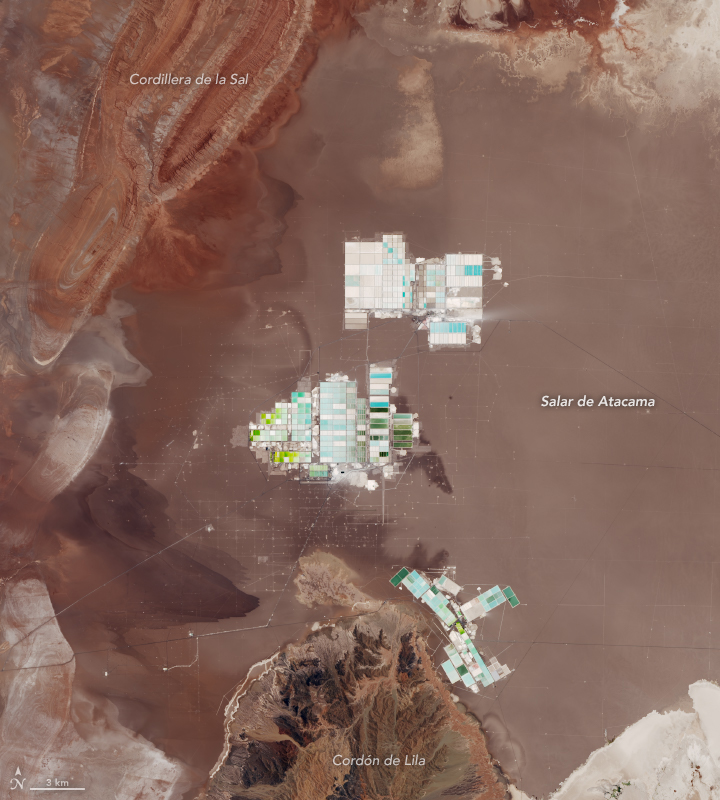
\includegraphics[width=0.48\linewidth]{images/book2/atacama-ponds.jpg}

{\small Evaporation ponds of lithium brine on the Salar de Atacama, seen
from orbit (Landsat 8, 2018; NASA Earth Observatory, public domain,
Wikimedia Commons). The colour of each pond changes as the brine
concentrates and salts crystallise.}
\end{omfigure}

\section{Hydrogen and the hydrides}

Hydrogen has one electron: it can lose it (\ce{H+}, carried by water as
\ce{H3O+}), share it (\omterm{def:b1:lewis-resonance-vsepr:lewis}{covalent bonds}), or gain one (\ce{H-}, with the
\omterm{def:b1:quantum-numbers:configuration}{electron configuration} of helium). Which it does depends on its partner.

\begin{definition}[Hydrides]\label{def:b1:s-block:hydride}
A \emph{hydride}\index{hydride} is a binary compound of hydrogen with
another element. \emph{Saline hydrides}\index{saline hydride}, formed
with the alkali and heavier \omterm{def:b1:s-block:families}{alkaline-earth metals} (\ce{LiH}, \ce{NaH},
\ce{CaH2}), are ionic solids containing \ce{H-}. \emph{Covalent
hydrides}\index{covalent hydride}, formed with the \omterm{def:b1:periodicity:table}{p-block} elements
(\ce{CH4}, \ce{NH3}, \ce{H2O}, \ce{HCl}), are molecular. \emph{Metallic
hydrides}\index{metallic hydride}, formed with some transition metals,
are solids in which hydrogen occupies \omterm{def:b1:crystals-metals:site}{interstitial sites} of the metal
\omterm{def:b1:crystals-metals:lattice}{lattice}, often with a variable composition.
\end{definition}

The \omterm{def:b1:s-block:hydride}{hydride} ion is a very \omterm{def:b1:predominant-reaction:strong-acid}{strong base} and reducing agent: \omterm{def:b1:s-block:hydride}{saline hydrides}
react with water, \ce{NaH + H2O -> NaOH + H2}, and serve as drying agents
for solvents and as bases in organic synthesis (\cref{ch:b1:alcohol-activation}).
The \omterm{def:b1:s-block:hydride}{covalent hydrides} of the second \omterm{def:b1:periodicity:table}{period} show the trend in
\omterm{def:b1:periodicity:electronegativity}{electronegativity} across it: \ce{CH4} neither acidic nor basic, \ce{NH3}
basic, \ce{H2O} amphoteric, \ce{HF} acidic.

\section{The alkali metals}

\begin{definition}[Alkali and alkaline-earth metals]\label{def:b1:s-block:families}
The \emph{alkali metals}\index{alkali metal} (Li, Na, K, Rb, Cs, Fr) form
\omterm{def:b1:periodicity:table}{group} 1, with one valence electron \textit{ns}$^1$; the
\emph{alkaline-earth metals}\index{alkaline-earth metal} (Be, Mg, Ca, Sr,
Ba, Ra) form \omterm{def:b1:periodicity:table}{group} 2, with \textit{ns}$^2$. Their elements are the
\omterm{def:b1:periodicity:table}{s-block}.
\end{definition}

\begin{proposition}[The alkali metals are strong reductants]\label{prop:b1:s-block:reducing-power}
The \omterm{def:b1:s-block:families}{alkali metals} have the lowest first ionisation energies of their
\omterm{def:b1:periodicity:table}{periods} (Li \qty{5.39}{eV}, Na 5.14, K 4.34) and very negative \omterm{def:b1:nernst:electrode-potential}{standard
potentials} (\ce{Li+}/\ce{Li} $-3.04$~V, \ce{Na+}/\ce{Na} $-2.71$,
\ce{K+}/\ce{K} $-2.94$): they reduce water and are found in nature only as
\ce{M+} ions.
\end{proposition}
% ledger: ie:Li, ie:Na, ie:K (E0 computed in figdata/bachelor-1/standard-potentials.py)

\begin{proof}
A single electron outside a noble-gas core, far from the nucleus and
screened by the inner shells (\cref{ch:b1:periodicity}), is easily
removed. In water the small \ce{M+} ion is strongly hydrated, which makes
the couple potential even lower. With $E^\circ$ more than \qty{2.2}{V}
below the line of water at pH 7 ($-0.41$~V), the reaction
\ce{2M + 2H2O -> 2M+ + 2OH- + H2} has an enormous constant
(\cref{prop:b1:nernst:equilibrium-constant}).
\end{proof}

\begin{omfigure}
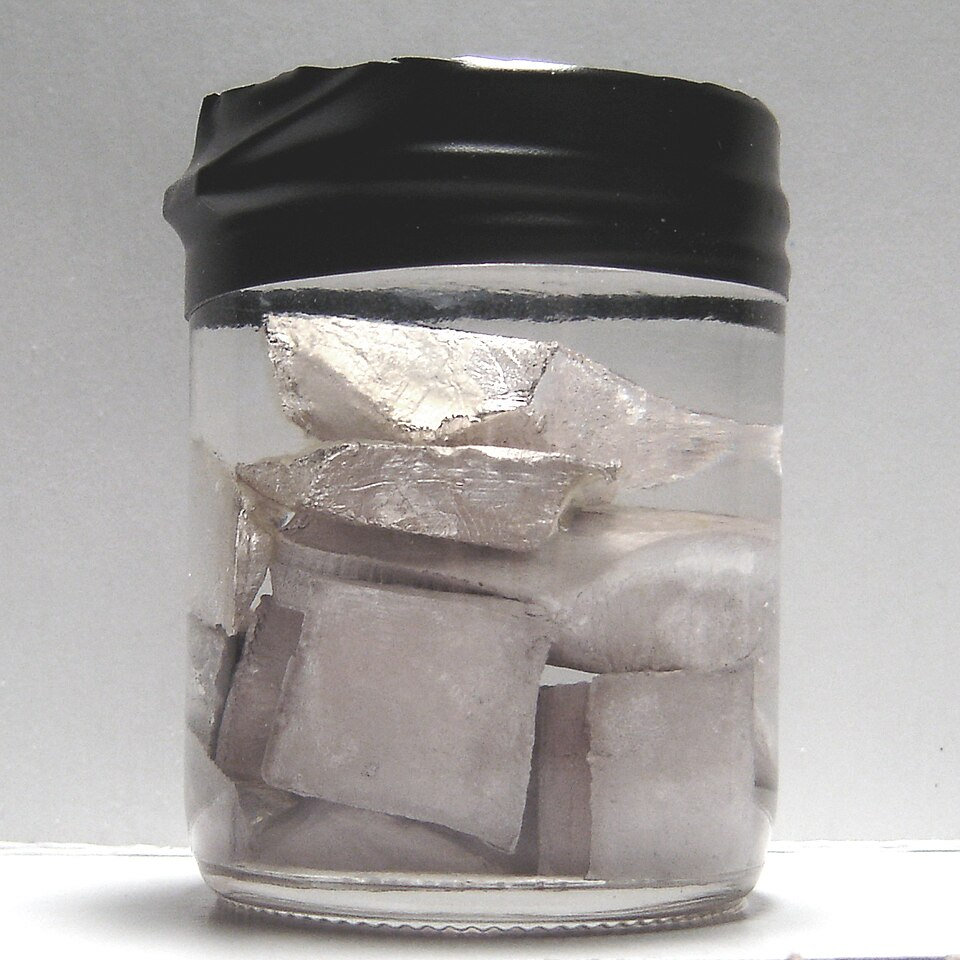
\includegraphics[height=4.6cm]{images/book2/sodium-oil.jpg}\hspace{0.8em}%
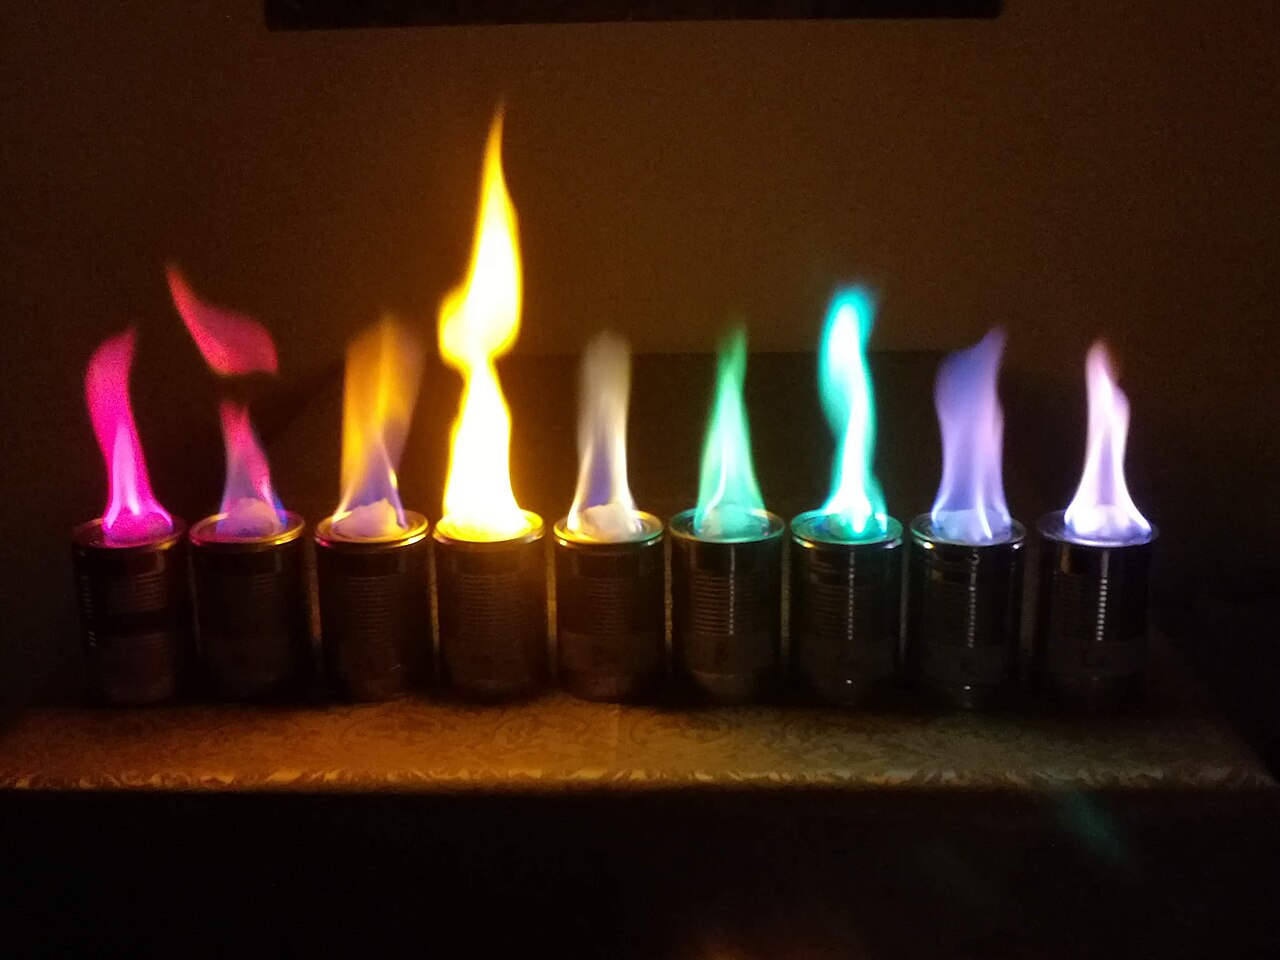
\includegraphics[height=4.6cm]{images/book2/flame-colours.jpg}

{\small Left: sodium is kept under mineral oil, away from air and moisture
(photograph Justin Urgitis, CC BY-SA 2.5). Right: flame colours, from left
to right, of lithium, strontium, calcium, sodium, barium, boron, copper,
caesium and potassium compounds: electrons excited in the flame return to
lower levels emitting light at wavelengths characteristic of each element
(\cref{ch:b1:quantum-numbers}) (photograph Hegelrast, CC BY-SA 4.0). Both
Wikimedia Commons.}
\end{omfigure}

\begin{inthelab}[A demonstration, not an experiment]
The reaction of sodium with water is shown only by a teacher, behind a
safety screen, with a piece the size of a lentil dropped into a large
trough of water containing phenolphthalein: the metal melts into a
running ball, hydrogen fizzes, and the pink trail shows the hydroxide
formed. Potassium ignites the hydrogen. Larger pieces explode. Sodium is
cut under oil, handled with tongs, and its residues destroyed with
ethanol, never with water.
\end{inthelab}

Lithium is the exception of its group: the smallest ion, the most
strongly hydrated, hence the most negative potential, yet the slowest to
react with water. Its compounds resemble those of magnesium (lithium
carbonate and phosphate are sparingly soluble, as magnesium's are), a
diagonal relationship across the periodic table. The \omterm{def:b1:s-block:families}{alkali metals} are
produced by electrolysis of their molten chlorides, since no chemical
\omterm{def:b1:nernst:couple}{reductant} is strong enough; the electrode reactions of such cells are
studied in the Year~2 volume.

\section{Sodium compounds in industry}

\begin{definition}[Character of oxides]\label{def:b1:s-block:oxide-character}
A \emph{basic oxide}\index{basic oxide} reacts with water to give a
hydroxide, or with acids to give salts (\ce{Na2O}, \ce{CaO}); an
\emph{acidic oxide}\index{acidic oxide} reacts with water to give an acid,
or with bases to give salts (\ce{CO2}, \ce{SO3}, \ce{P4O10}); an
\emph{amphoteric oxide}\index{amphoteric oxide} reacts with both acids and
bases (\ce{Al2O3}, \ce{ZnO}). Across a \omterm{def:b1:periodicity:table}{period}, oxides go from basic
(metals, left) to acidic (non-metals, right).
\end{definition}

Sodium hydroxide is made by electrolysis of brine (the chlor-alkali
process, which also \omterm{def:b1:extent-q-and-k:fractional-extent}{yields} chlorine and hydrogen). Sodium carbonate, soda
ash, used for glass, detergents and lithium extraction, is either mined
as the mineral trona or made from salt and limestone: in 2025 the world
produced about 71 million tonnes, 19 million from natural deposits and 52
million synthetic, most of it by the Solvay process.
% ledger: usgs:sodaash-total-2025, usgs:sodaash-natural-2025, usgs:sodaash-synthetic-2025

\begin{proposition}[The Solvay process]\label{prop:b1:s-block:solvay}
The Solvay process converts sodium chloride and calcium carbonate into
sodium carbonate and calcium chloride, \ce{2NaCl + CaCO3 -> Na2CO3 +
CaCl2}, through steps in which ammonia and carbon dioxide are recycled.
\end{proposition}

\begin{proof}
The steps are: (1) \ce{CaCO3 -> CaO + CO2} (kiln); (2) \ce{NaCl + NH3 +
CO2 + H2O -> NaHCO3 + NH4Cl} (carbonation of ammoniacal brine; the
hydrogencarbonate, the least soluble salt present, precipitates); (3)
\ce{2NaHCO3 -> Na2CO3 + CO2 + H2O} (calcination); (4) \ce{CaO + H2O ->
Ca(OH)2}; (5) \ce{Ca(OH)2 + 2NH4Cl -> CaCl2 + 2NH3 + 2H2O} (ammonia
recovery). Adding $(1) + 2\times(2) + (3) + (4) + (5)$, the \ce{NH3},
\ce{CO2}, \ce{NH4Cl}, \ce{NaHCO3}, \ce{CaO}, \ce{Ca(OH)2} and water cancel:
\ce{2NaCl + CaCO3 -> Na2CO3 + CaCl2}.
\end{proof}

\begin{omfigure}
\begin{tikzpicture}[font=\small, >={Stealth}, box/.style={draw, rounded corners, fill=omDef!8, minimum width=2.6cm, minimum height=0.8cm, align=center}]
  \node[box] (kiln) at (0,0) {lime kiln\\\ce{CaCO3 -> CaO + CO2}};
  \node[box] (tower) at (5.3,0) {carbonation tower\\\ce{NaHCO3} precipitates};
  \node[box] (calc) at (10.2,0) {calciner\\\ce{NaHCO3} $\to$ \ce{Na2CO3}};
  \node[box] (slake) at (0,-2.6) {slaker\\\ce{CaO + H2O -> Ca(OH)2}};
  \node[box] (still) at (5.3,-2.6) {ammonia still\\\ce{NH4Cl + Ca(OH)2}};
  \draw[->, thick] (kiln) -- node[above] {\ce{CO2}} (tower);
  \draw[->, thick] (tower) -- node[above, font=\scriptsize] {\ce{NaHCO3}} (calc);
  \draw[->, thick] (calc.north) -- ++(0,0.6) -| node[pos=0.25, above] {\ce{CO2} recycled} (tower.north);
  \draw[->, thick] (kiln) -- node[left] {\ce{CaO}} (slake);
  \draw[->, thick] (slake) -- node[above, font=\scriptsize] {\ce{Ca(OH)2}} (still);
  \draw[->, thick] (tower) -- node[right] {\ce{NH4Cl}} (still);
  \draw[->, thick] (still.east) -- ++(1.2,0) |- node[pos=0.25, right] {\ce{NH3} recycled} ($(tower.east)+(0,-0.25)$);
  \draw[<-, thick] (tower.north west) -- ++(-0.5,0.6) node[above] {brine \ce{NaCl}};
  \draw[->, thick] (calc.east) -- ++(0.8,0) node[right] {\ce{Na2CO3}};
  \draw[->, thick] (still.south) -- ++(0,-0.6) node[below] {\ce{CaCl2}};
\end{tikzpicture}

{\small The Solvay process. Carbon dioxide and ammonia go round in loops;
salt and limestone enter, soda ash and calcium chloride leave.}
\end{omfigure}

\begin{omfigure}
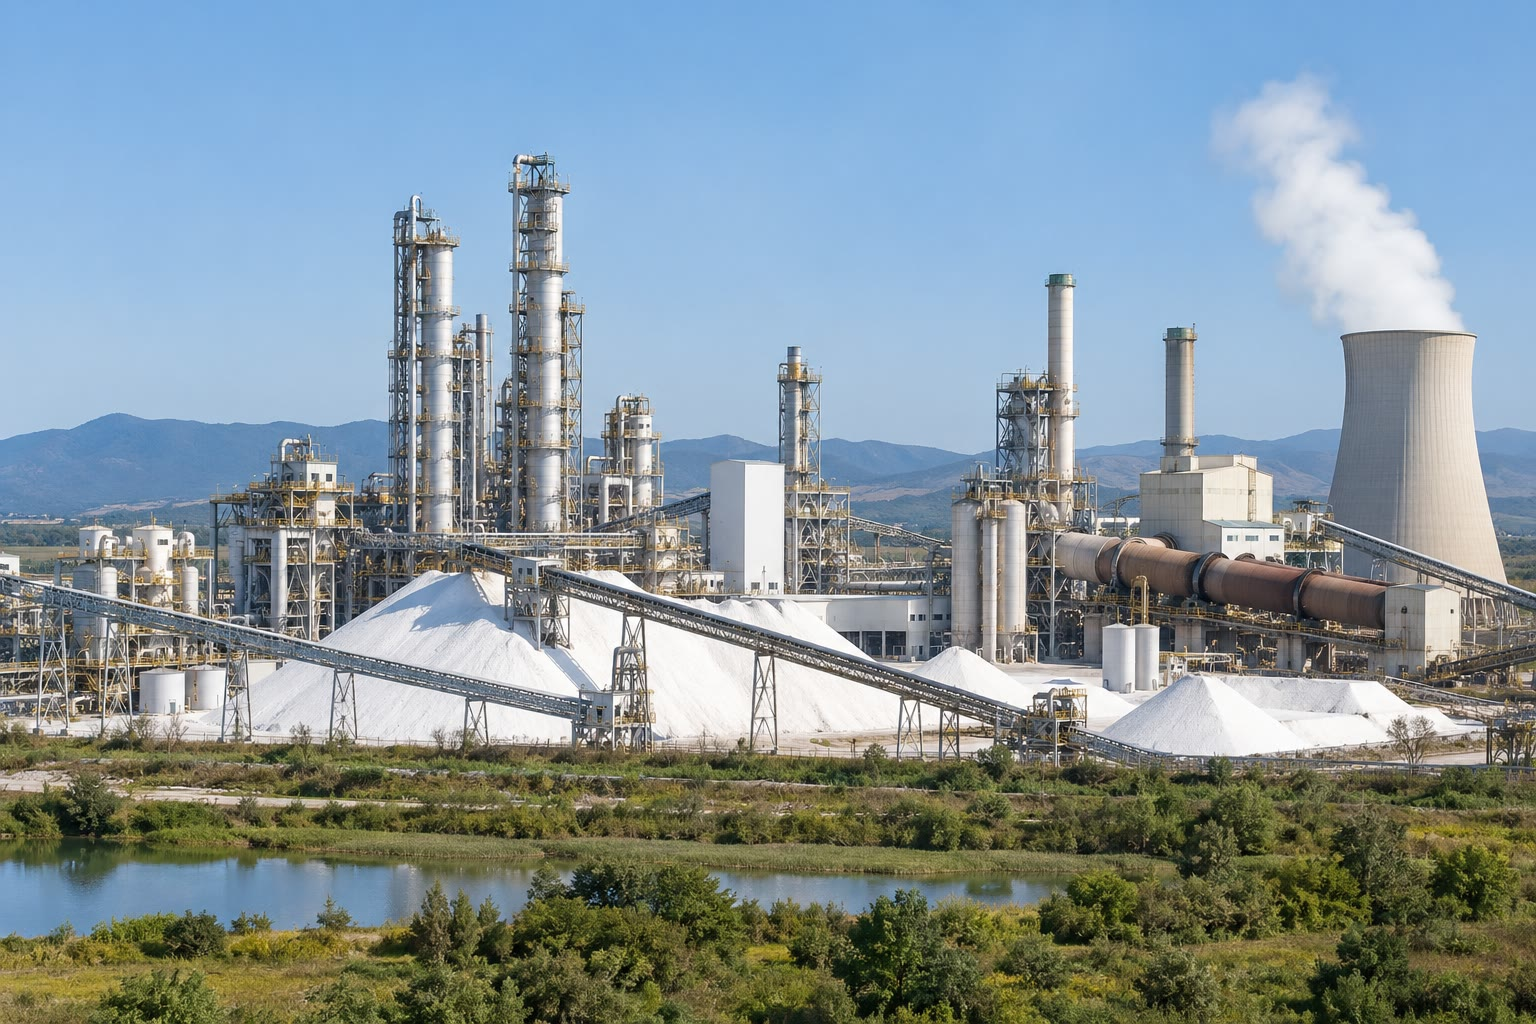
\includegraphics[width=0.55\linewidth]{images/book2/ai/b1-26-soda-ash-plant.jpg}

{\small A soda-ash plant: lime kilns, carbonation towers and stockpiles of
sodium carbonate.}
\end{omfigure}

\begin{method}[Mass balance on a flow sheet]\label{met:b1:s-block:mass-balance}
\begin{enumerate}
  \item Write the overall equation (sum of the steps, recycled species
        cancelled).
  \item From the product wanted, compute the amounts of raw materials
        with the overall equation, then correct for the \omterm{def:b1:extent-q-and-k:fractional-extent}{yield} of each step.
  \item For a recycled species, compute only the make-up needed to replace
        its losses.
  \item Check the balance of each element between inputs and outputs.
\end{enumerate}
\end{method}

\section{The alkaline-earth metals}

Magnesium and calcium are less reactive than the \omterm{def:b1:s-block:families}{alkali metals} (higher
ionisation energies: Mg \qty{7.65}{eV}, Ca 6.11; two electrons to lose) but
still strong \omterm{def:b1:nernst:couple}{reductants} ($E^\circ$ of \ce{Mg^2+}/\ce{Mg} $-2.36$~V).
Magnesium burns in air with a dazzling white light; its oxide film
protects it at room temperature. Magnesium is recovered from sea water by
precipitating its hydroxide with lime, $\mathrm{p}K_s = 11.25$
(\cref{ch:b1:precipitation}).
% ledger: ie:Mg, ie:Ca

\begin{proposition}[The lime cycle]\label{prop:b1:s-block:lime-cycle}
Limestone, quicklime, slaked lime and limestone again form a cycle:
\ce{CaCO3 -> CaO + CO2} (heated in a kiln); \ce{CaO + H2O -> Ca(OH)2}
(slaking, strongly exothermic); \ce{Ca(OH)2 + CO2 -> CaCO3 + H2O} (setting
of lime mortar in air). The cycle as a whole changes nothing chemically,
but stores and releases energy and carbon dioxide.
\end{proposition}

\begin{proof}
Adding the three equations, every species cancels. The decomposition of
the carbonate requires heat, released again in the two other steps; the
\ce{CO2} given off in the kiln is taken up again, slowly, by the mortar.
\end{proof}

\begin{omfigure}
\begin{tikzpicture}[font=\small, >={Stealth}]
  \node[draw, rounded corners, fill=omDef!8] (a) at (90:2.0) {\ce{CaCO3} limestone};
  \node[draw, rounded corners, fill=omDef!8] (b) at (-30:2.0) {\ce{CaO} quicklime};
  \node[draw, rounded corners, fill=omDef!8] (c) at (210:2.0) {\ce{Ca(OH)2} slaked lime};
  \draw[->, thick] (a) to[bend left=25] node[right, align=left] {heat\\$-\ce{CO2}$} (b);
  \draw[->, thick] (b) to[bend left=25] node[below] {$+\ce{H2O}$} (c);
  \draw[->, thick] (c) to[bend left=25] node[left, align=right] {$+\ce{CO2}$\\$-\ce{H2O}$} (a);
\end{tikzpicture}

{\small The lime cycle, from limestone to mortar and back to calcium
carbonate.}
\end{omfigure}

\section{Lithium}

\begin{omfigure}
\begin{tikzpicture}
\begin{axis}[
  xbar, width=0.78\linewidth, height=5.4cm, xmin=0, xmax=110,
  symbolic y coords={CA,ML,BR,AR,ZW,CL,CN,AU}, ytick=data,
  yticklabels={Canada, Mali, Brazil, Argentina, Zimbabwe, Chile, China, Australia},
  xlabel={lithium mined in 2025 (thousand tonnes of Li, estimates)}, bar width=8pt,
  nodes near coords, every node near coord/.append style={font=\scriptsize},
  tick label style={font=\small}, label style={font=\small}, enlarge y limits=0.1]
\addplot[fill=omDef!45, draw=omDef] coordinates {(5.6,CA) (9.4,ML) (12,BR) (23,AR) (28,ZW) (56,CL) (62,CN) (92,AU)};
\end{axis}
\end{tikzpicture}

{\small The largest lithium producers in 2025 (estimates; world total
about \num{290000} tonnes of lithium). Australia mines hard rock
(spodumene); Chile and Argentina pump brines.}
% ledger: usgs:li-canada-2025, usgs:li-mali-2025, usgs:li-brazil-2025, usgs:li-argentina-2025, usgs:li-zimbabwe-2025, usgs:li-chile-2025, usgs:li-china-2025, usgs:li-australia-2025, usgs:li-world-2025
\end{omfigure}

Brine is concentrated by evaporation, magnesium removed with lime, and
lithium carbonate precipitated with soda ash. Lithium carbonate has the
unusual property of being less soluble hot than cold: \qty{1.31}{\percent}
by mass at \qty{20}{\celsius}, \qty{0.84}{\percent} at \qty{80}{\celsius},
\qty{0.71}{\percent} at \qty{100}{\celsius}. It is therefore precipitated
from hot solution, as the weekend problem computes.
% ledger: sol:Li2CO3-20, sol:Li2CO3-80, sol:Li2CO3-100

\section{Exercises}

\begin{exercise}[$\star$]\label{exo:b1:s-block:1}
Classify as saline, covalent or \omterm{def:b1:s-block:hydride}{metallic hydride}: \ce{KH}, \ce{SiH4},
\ce{CaH2}, \ce{H2S}, \ce{PdH_{0.6}}. Write the reaction of \ce{CaH2} with water.
\end{exercise}

\begin{exercise}[$\star$]\label{exo:b1:s-block:2}
Write the reactions of lithium, sodium and potassium with water, and of
magnesium with dilute hydrochloric acid.
\end{exercise}

\begin{exercise}[$\star$]\label{exo:b1:s-block:3}
Classify as basic, acidic or amphoteric: \ce{Na2O}, \ce{MgO}, \ce{Al2O3},
\ce{SiO2}, \ce{SO3}, \ce{ZnO}, \ce{CO2}. Write one reaction for each kind.
\end{exercise}

\begin{exercise}[$\star$]\label{exo:b1:s-block:4}
Compute the constant of \ce{2Na + 2H2O -> 2Na+ + 2OH- + H2} at pH 14 from the
\omterm{def:b1:nernst:electrode-potential}{standard potentials}.
\end{exercise}

\begin{exercise}[$\star\star$]\label{exo:b1:s-block:5}
Explain the flame colours of lithium (red) and sodium (yellow) using the
\omterm{def:b1:quantum-numbers:energy-level}{energy levels} of atoms (\cref{ch:b1:quantum-numbers}). What is the energy
of a yellow photon at \qty{589}{nm}?
\end{exercise}

\begin{exercise}[$\star\star$]\label{exo:b1:s-block:6}
Compute the mass of limestone (pure \ce{CaCO3}) and of sodium chloride
needed for one tonne of soda ash by the Solvay process, with an overall
\omterm{def:b1:extent-q-and-k:fractional-extent}{yield} of \qty{90}{\percent} on sodium chloride.
\end{exercise}

\begin{exercise}[$\star\star$]\label{exo:b1:s-block:7}
Sea water contains about \qty{1.3}{g/L} of magnesium (data of the
exercise). At what pH does magnesium hydroxide begin to precipitate?
What mass of slaked lime precipitates the magnesium of \qty{1.0}{m^3}?
\end{exercise}

\begin{exercise}[$\star\star$]\label{exo:b1:s-block:8}
Why does lithium react more slowly with water than potassium, although
its \omterm{def:b1:nernst:electrode-potential}{standard potential} is lower? Distinguish thermodynamics and kinetics.
\end{exercise}

\begin{exercise}[$\star\star$]\label{exo:b1:s-block:9}
Compute the mass of quicklime obtained from one tonne of limestone and the
volume of \ce{CO2} released, at \qty{25}{\celsius} and \qty{1}{bar}.
\end{exercise}

\begin{exercise}[$\star\star\star$]\label{exo:b1:s-block:10}
The world mined about \num{290000} tonnes of lithium in 2025. What mass of
lithium carbonate is that? If a car battery holds \qty{8}{kg} of
lithium (data of the exercise), how many batteries could it supply?
\end{exercise}

\begin{exercise}[$\star\star\star$]\label{exo:b1:s-block:11}
Show that the \omterm{def:b1:precipitation:solubility}{solubility} of lithium carbonate falls with temperature from
the data of the chapter, and explain why precipitating it hot improves the
recovery from a brine.
\end{exercise}

\begin{exercise}[$\star\star\star$]\label{exo:b1:s-block:12}
In step (2) of the Solvay process, the solution contains \ce{Na+},
\ce{NH4+}, \ce{Cl-} and \ce{HCO3-}. Explain why sodium hydrogencarbonate
precipitates rather than ammonium chloride, and why the process needs
ammonia rather than sodium hydroxide.
\end{exercise}

\section{Problem: Lithium from Brine}

\begin{problem}[{Weekend problem --- concentrating a lithium brine,
removing magnesium with lime, precipitating lithium carbonate with soda
ash, and the mass of lithium carbonate recovered from one cubic metre}]
\label{pb:b1:s-block:1}
A brine pumped from under a salt flat contains \qty{1.5}{g/L} of lithium
and \qty{0.60}{g/L} of magnesium (as ions, with much sodium chloride).
Evaporation in ponds concentrates it four times. One cubic metre of the
concentrated brine is then treated: lime removes the magnesium, soda ash
the calcium, and hot soda ash finally precipitates lithium carbonate at
\qty{80}{\celsius}. Data: molar masses (\unit{g/mol}) Li 6.9, Mg 24.3,
\ce{Ca(OH)2} 74.1, \ce{Na2CO3} 106.0, \ce{Li2CO3} 73.8; $\mathrm{p}K_s$
\ce{Mg(OH)2} 11.25, \ce{CaCO3} 8.30; $\mathrm{p}K_e = 14.00$; \omterm{def:b1:precipitation:solubility}{solubility}
of \ce{Li2CO3} \qty{0.84}{\percent} by mass at \qty{80}{\celsius}; take
the final liquor as \qty{1.00}{m^3} of density \qty{1.0}{kg/L}.

\medskip
\noindent\textbf{Part I --- Concentrating.}
\begin{enumerate}
  \item Compute the concentrations of lithium and magnesium in the
        concentrated brine.
  \item What volume of water evaporates per cubic metre of concentrated
        brine?
  \item Why is solar evaporation used rather than heating?
  \item Which salt crystallises first in the ponds, and why?
  \item Compute the amounts of lithium and magnesium in one cubic metre.
  \item Why must magnesium be removed before lithium is precipitated?
\end{enumerate}

\medskip
\noindent\textbf{Part II --- Removing magnesium and calcium.}
\begin{enumerate}[resume]
  \item Write the reaction of magnesium ions with slaked lime.
  \item Compute the mass of slaked lime needed (stoichiometric).
  \item At what pH is \qty{99.9}{\percent} of the magnesium precipitated?
  \item Why is lithium not precipitated as its hydroxide?
  \item Write the removal of the calcium introduced, with soda ash.
  \item Compute the mass of soda ash needed for that step.
\end{enumerate}

\medskip
\noindent\textbf{Part III --- Lithium carbonate.}
\begin{enumerate}[resume]
  \item Write the precipitation of lithium carbonate.
  \item Compute the mass of soda ash needed for the lithium.
  \item Compute the theoretical mass of lithium carbonate.
  \item Why is the precipitation done at \qty{80}{\celsius}?
  \item What mass of lithium carbonate stays dissolved in the liquor?
  \item How is the precipitate washed without losing much of it?
\end{enumerate}

\medskip
\noindent\textbf{Part IV --- Balance.}
\begin{enumerate}[resume]
  \item Compute the mass of lithium carbonate recovered.
  \item Compute the recovery of lithium.
  \item Suggest what is done with the liquor.
  \item Compare the lithium in one cubic metre with the world production
        of 2025: how many cubic metres would that production represent?
  \item State the mass of lithium carbonate recovered per cubic metre of
        concentrated brine.
\end{enumerate}
\end{problem}
